\documentclass{article} % For LaTeX2e
\usepackage{nips13submit_e,times}
\usepackage{hyperref}
\usepackage{url}
\usepackage{amsmath}
\usepackage{amssymb}
\usepackage{natbib}
\usepackage[pdftex]{graphicx}
%\documentstyle[nips13submit_09,times,art10]{article} % For LaTeX 2.09

% \DeclareMathOperator{\Sample}{Sample}
\let\vaccent=\v % rename builtin command \v{} to \vaccent{}
\renewcommand{\v}[1]{\ensuremath{\mathbf{#1}}} % for vectors
\newcommand{\gv}[1]{\ensuremath{\mbox{\boldmath$ #1 $}}} 
% for vectors of Greek letters
\newcommand{\uv}[1]{\ensuremath{\mathbf{\hat{#1}}}} % for unit vector

\let\underdot=\d % rename builtin command \d{} to \underdot{}
\renewcommand{\d}[2]{\frac{d #1}{d #2}} % for derivatives
\newcommand{\dd}[2]{\frac{d^2 #1}{d #2^2}} % for double derivatives
\newcommand{\pd}[2]{\frac{\partial #1}{\partial #2}} 
% for partial derivatives
\newcommand{\pdd}[2]{\frac{\partial^2 #1}{\partial #2^2}} 
% for double partial derivatives
\newcommand{\pdc}[3]{\left( \frac{\partial #1}{\partial #2}
 \right)_{#3}} % for thermodynamic partial derivatives
\newcommand{\ket}[1]{\left| #1 \right>} % for Dirac bras
\newcommand{\bra}[1]{\left< #1 \right|} % for Dirac kets
\newcommand{\braket}[2]{\left< #1 \vphantom{#2} \right|
 \left. #2 \vphantom{#1} \right>} % for Dirac brackets
\newcommand{\matrixel}[3]{\left< #1 \vphantom{#2#3} \right|
 #2 \left| #3 \vphantom{#1#2} \right>} % for Dirac matrix elements

\newcommand{\exval}[1]{\left\langle #1 \right\rangle} % for angle-bracket expectation values

\newcommand{\abv}[1]{\lvert #1 \rvert} % for absolute values

\title{Criticality in neural networks paper title}


\author{
Paul Rozdeba%\thanks{ Use footnote for providing further information
%about author (webpage, alternative address)---\emph{not} for acknowledging
%funding agencies.} \\
\\
Department of Physics\\
University of California, San Diego\\
La Jolla, CA 92093 \\
\texttt{prozdeba@physics.ucsd.edu} \\
\And
Forrest Sheldon \\
Department of Physics\\
University of California, San Diego\\
La Jolla, CA 92093 \\
\texttt{fsheldon@physics.ucsd.edu} \\
}

% The \author macro works with any number of authors. There are two commands
% used to separate the names and addresses of multiple authors: \And and \AND.
%
% Using \And between authors leaves it to \LaTeX{} to determine where to break
% the lines. Using \AND forces a linebreak at that point. So, if \LaTeX{}
% puts 3 of 4 authors names on the first line, and the last on the second
% line, try using \AND instead of \And before the third author name.

\newcommand{\fix}{\marginpar{FIX}}
\newcommand{\new}{\marginpar{NEW}}

\nipsfinalcopy % Uncomment for camera-ready version

\begin{document}
\maketitle

%-------------------------------------------------------------------------------
% ABSTRACT
%-------------------------------------------------------------------------------
\begin{abstract}
It has been posited that biological neural networks, such as a brain, may
naturally exist in critical states.  We propose two mechanisms for signal
transduction in two such networks as encoding strategies which are optimized by
criticality.  First, we examine compressive sensing in a 2-dimensional Ising
model at or near its critical temperature.  Secondly, we examine the dynamical
synchronization capabilities of a random neural network model as it transitions
into chaotic behavior.  We propose that both techniques should be most successful
at the critical state of either model.
\end{abstract}

%-------------------------------------------------------------------------------
% Introduction
%-------------------------------------------------------------------------------
\section{Introduction}
Criticality has enjoyed widespread success in the scientific community, being
applied to problems as diverse as gene expression, starling flocks, and forest
fires.\cite{Chialvo2010}  Originating in statistical physics, criticality is a set
of properties of a system near a second order phase transition, in which the
system possesses long range correlations in both space and time.  These
properties make it an attractive tool for describing the many complex systems
that seem to display similar long range order.  However, their analytical
intractability restricts most arguments for criticality's existence to a
rather superficial resemblence, usually resting on the existence of a power
law in some measurement of the system. The recent realization that power laws
occur far more often, and for a broader range of mechanisms than originally
thought has tempered some of the enthusiasm for scale-free networks and, by
association, criticality.\cite{Keller2005} However, as the most established and
flexible phenomenon displaying long range order, criticality still occupies
a strong position as a candidate theory for understanding complex systems.

In the review  "Emergent complex neural dynamics\cite{Chialvo2010}" Dante Chialvo
makes a case for the brain exhibiting criticality.  He pulls from several
pieces of evidence including:
\begin{itemize}
\item The brain contains the \emph{necessary} elements (a large network of
nonlinear interacting elements) to display complex emergent behavior and thus
criticality.
\item EEG/MEG readings of healthy brains do not show a preferred time scale.
\item All models that display emergent complex behavior also display
criticality. 
\item Neuronal avalanches have a scale free size distribution matching a
critical branching process.
\item Degree distributions created from fMRI recordings are scale-free.
\end{itemize}
Taken as a whole these form a reasonably strong case for criticality playing 
some role in the brain's dynamics however they all suffer from the defect
mentioned previously: Power laws are nonspecific to criticality.  As such, we
take up the same investigation from the opposite direction asking 'Why would a
brain want to be critical?'  To this end, we examine systems that possess a
known critical phase transition and which are relevant to neuroscience: the
ising model and a simple neural network with a leak current and sigmoidal
connection strengths.

In the Ising model, we examine the structure of clustering that occurs in the
vicinity of a phase transition.  In particular, is it possible to reconstruct
the states of distant spins held fixed as the system is evolved, given the state
of the system at all points between them?  We examine this possibility at
various temperatures and examine the independence of multiple measurements.

%-------------------------------------------------------------------------------
% FORREST'S SECTION
%-------------------------------------------------------------------------------
\section{The Ising Model}
The ising model could be considered the canonical physical system exhibiting
critical phase transition.  The spins may be considered small arrows that may
point up or down with a corresponding value of +1 and -1. They are governed by
the Hamiltonian,
\[H = -\frac{\epsilon}{2} \sum_{i\neq j} s_i s_j\]
where $\epsilon$ is some energy scale and the factor of $\frac{1}{2}$
compensates for double counting in the sum.  There is an energetic cost for two
neighboring spins to oppose each other.  As such, the system displays two phases:
As the temperature is raised, the system moves from an ordered phase in which
all of the spins point in the same direction and thus minimize the energy, to a
disordered phase in which neighboring spins oppose each other. Between the two
phases the system displays power law correlation distributions in space and time
and a large number of accessible states.  These three regimes are displayed in
Figure 1.
\begin{figure}[h]
\begin{center}
\includegraphics[width=0.5\linewidth]{Ising_states.png}
\end{center}
\caption{The ising model below, near, and above the critical temperature}
\end{figure}

\section{Compressive Sensing}
Compressive sensing is a process by which a $k$-sparse signal of length $N$ may
be perfectly reconstructed from only $O(K\log{N/K})$ measurements if those
measurements are random projections.\cite{Candes2008} This
is interesting both because $O(K\log{N/K})$ is much better than $O(N)$ which is
implied by the Shannon-Nyquist theorem, and that this is done using random
projections.  This is because random projections are information preserving in
that they approximately preserve distances between major features in the data.
Stating this more mathematically, given a discrete signal $x$ with a sparse
representation in some basis $\Psi$, we acquire $x$ by projecting it onto a set
of vectors $\Phi$, acquiring a vector of projections $y$:
\[y = \Phi x = \Phi \Psi s = \Theta s\]
We can perfectly reconstruct our original signal $s$ from only a few
measurements $y$ so long as $\Theta = \Phi\Psi$ obeys the \emph{Restricted
Isometry Property} which happens to be fulfilled by most random bases.
(Interested readers may consult\cite{Candes2008}\cite{Baraniuk2007}) The sparsity of
most natural signals and the use of random projections has led Chuck Stevens to
suggest that this coding strategy may be used in a modified form in several
regions of the cortex that have resisted attempts at making a 'map' of their
function.  We propose that a system at criticality may naturally perform these
projections and choose an Ising model to attempt to demonstrate it.

\section{Methods-I}
Ising models were simulated by means of markov chain monte carlo.
\cite{MacKay2003}\cite{Schroeder1999} Comparison
between Metropolis and Gibbs sampling algorithms yielded that the Metropolis
algorithm performed poorly at high temperatures and Gibbs sampling was
performed thereafter.  A signal vector $\vec{s}$ was generate with [-1, 1] entries. These
entries were inputed into the model at random points, held fixed as the system
evolved. A single random spin $r$ was also selected to be recorded. We would regard
this single spin as our random projection of the signal held fixed in the model.
 After evolving the system to equilibrium, a breadth first search was performed
through the cluster in the model containing the recording spin.  A cluster
incidence vector $\vec{i}$ was formed whose elements were 1 if the corresponding signal
element was a member of the cluster and zero otherwise.  The signal vector was
then $l^1$ normalized so that the equation, $r = \vec{i} \cdot \vec{s}$ was satisfied.  By
repeating this procedure with the signal spins held fixed and the same recording
spin, we were able to generate a system $\vec{r} = I\vec{s}$ that should be approximately
solved by our signal vector and recorded spins.

A full study of the properties of these measurement vectors (and alternative
schemes at constructing a measurement matrix) is still underway.  Under the
limitation of time, two analyses were undertaken.  First, the rank of $I$ was
examined as a function of number of measurements and temperature. Second, the
system was solved by means of the Moore-Penrose pseudoinverse and the reconstruction
error calculated, also as a function of number of measurements and temperature.
All results here are for a $(32\times 32)$ spin model to keep computation time
reasonable, although similar analyses have been run on larger systems.

\section{Results-I}

Results thus far have been...a bit mundane.  We begin with the high point.  The
rank of the measurement matrix (Figure 2) seems to show a distinct temperature dependence.
At the critical temperature, each measurement remains independent and the
measurement matrix attains full row rank in as few steps as possible.  Only
slightly worse is the low temperature limit.  Here several measurement vectors are
linearly dependent on those previously measured and do not increase the rank.
Finally, worst off is the high temperature limit in which the matrix was not able
to reach full rank given twice as many measurements as necessary.
\begin{figure}[h]
\begin{center}
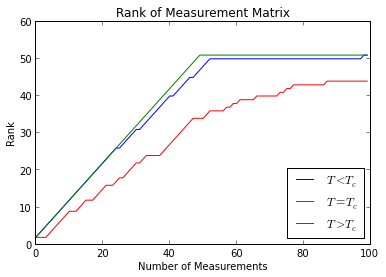
\includegraphics[width=0.5\linewidth]{Ranks.png}
\end{center}
\caption{Measurement matrix ranks at various temperatures}
\end{figure}
This would seem to indicate that the critical state offers some advantage over its
neighboring phases in its ability to transmit information located around the model.
In the disordered phase, the small correlation length makes it very difficult to
obtain interactions with distant spins, and in the ordered phase the large interaction
size causes repetitive couplings to all the spins also transmitting redundant information.

Attempting to reconstruct the original signal from these measurement however, has
been far less successful.  Using the Moore-Penrose pseudoinverse to attempt
reconstruction at every step, we were able to calculate reconstruction error
for each measurement (Figure 3).  
\begin{figure}[h]
\begin{center}
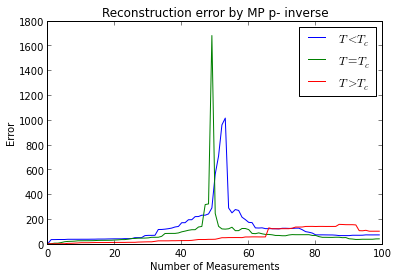
\includegraphics[width=0.5\linewidth]{errors.png}
\end{center}
\caption{Reconstruction error at various temperatures}
\end{figure}
We have far less understanding this figure.  It seems that the critical temperature
is the most numerically unstable of all and especially so just as the matrix reaches
full rank.  As this is the case for the low temperature matrix as well, this may be
a feature of the MP pseudoinverse.  While an $l^1$ minimization would have been more
enkeeping with the original inspiration for this project due to its preferred role
in compressive sensing, it is substantially more difficult to implement and refinements
of the reconstruction will be relegated to subsequent work. As it stands, I believe
the poor quality of the reconstructions is feature of the specific encoding and 
reconstruction scheme used and that further work may yield subsantially more accurate results.
%-------------------------------------------------------------------------------
% PAUL'S SECTION
%-------------------------------------------------------------------------------
\section{Dynamical synchronization technique}
The model equations are coupled to a set of data through a linear term as
\begin{align}
	\d{x_i}{t} = f_i(x) + \sum_{j} g_{ij} \left(y_j - x_j\right)
\end{align}
where $x(t)$ and $y(t)$ are the model and the data trajectories, respectively, and $g_{ij}$ is a set of coupling constants.  In practice, only a few of the couplings will be nonzero (corresponding to the components of the system which can be measured) and the matrix $g_{ij}$ is diagonal, since in this scheme there is no obvious advantage to coupling different components of the system to each other.

In general, a model can be synchronized to a data set if enough measurements are made, and if the coupling is large enough.  What constitutes ``enough'' seems to come on a case-by-case basis.  Roughly, what is required is for the linear terms to regularize the (coupled) solution manifold by making the value of the largest Lyapunov exponent non-positive.  However, the ratio of the $i$-th coupling term to the $i$-th term of the dynamics must remain small, so as to not wash out the physicality of the problem (in practice, this may also increase the speed of convergence to the actual solution).  In other words, adjusting the coupling is a delicate balance for which there is no general procedure.

The success of the procedure, however, is not ultimately measured by the ability to synchronize, but by the ability of the model \emph{make predictions} after the coupling is turned off, since in general we're only able to measure a few components of the system.  In the case where we have access to all of the data states, however, we can additionally test the procedure by examining the normally unobservable states.  This is called a \emph{twin experiment} in the literature and is a useful technique for assessing the viability of the model to synchronize in a controlled setting.

\section{Random neural network model}
We now consider a neural network model, originally presented by \cite{Sompolinsky1988}, which is a dynamical system describing a network of $N$ randomly connected elements each having a leaky capacitive term.  The equations of motion describing the system are
\begin{align}
	\d{V_i}{t} &= -V_i + \sum_{j=1}^{N} J_{ij} \phi(V_j) \label{eq:m1_eom}
\end{align}
where $\phi(V_i)$ is a function which may be thought of as an ``activity'' proportional to the synaptic current between neurons $i$ and $j$.  One possible choice is a sigmoid function of $V$, i.e. $\phi_i = \tanh\left(\alpha V_i\right)$.  This choice is both biologically motivated as acting to saturate synaptic activity as a function of membrane voltage, as well as mathematically to avoid highly unstable, runaway solutions to eq. (\ref{eq:m1_eom}).  $\alpha$ acts as a control parameter on the turnaround rate of the synaptic activity around $V = 0$; in some sense it controls the ``degree of nonlinearity'' in the system.

The matrix $J_{ij}$ describes the connectivity in the network; in this particular model, $J_{ij}$ is chosen to be a Gaussian random matrix with elements distributed according to the statistics
\begin{align}
	\exval{J_{ij}} = 0, \quad \exval{J_{ij}J_{kl}} = \frac{\tilde{J}^2}{N} \: \delta_{ik}\delta_{jl} \left(1 - \delta_{ij}\right) \left(1 - \delta_{kl}\right) \label{eq:m1_stats}
\end{align}
which means synaptic connections are, in general, asymmetric and totally decorrelated.  This also means that, on average, half of the connections are inherently inhibitory and half are excitatory.  We use ``inherently'' because the sign of the synaptic current into neuron $i$ switches depending on the sign of $V_j$.

A detailed mathematical treatment of this model in the limit of large $N$ is given in \cite{Sompolinsky1988}.  Under the replacement $\alpha \rightarrow g\tilde{J}$ in the expression for $\phi(V_i)$, the model undergoes a ``phase transition'' when the control parameter $g\tilde{J}$ reaches a critical value of 1.  This is manifest in the structure of the attracting solution manifold in the $\{V_i\}$ state space, which acquires a positive Lyapunov exponent; in other words a family of chaotic solutions to (\ref{eq:m1_eom}) appears.

The similarity of this transition to the phase transition in the 2D Ising model near $T_\text{crit}$ is most apparent in the behavior of the quantity
\begin{align}
	\Delta(t) \equiv \exval{V_i(t_0) V_i(t_0 + t)} \label{eq:m1_Cteq}
\end{align}

\subsection{Numerical analysis}
We examined the model for $N=256$ neurons with a single instantiation of $J_{ij}$.  Ideally, we would like to scale up the simulation size to a larger $N$, perhaps near 1000, and to gather statistics about an \emph{ensemble} of models parameterized by different instantiations of $J_{ij}$.  However, limited by time, we now present said results as at least a preliminary examination of the model.

First, we performed a comparison of numerical results to the analytic results of \cite{Sompolinsky1988}.  For a single randomly drawn instantiation of $J_{ij}$, (\ref{eq:m1_eom}) was integrated forward in time using the \texttt{LSODA} solver in \texttt{scipy.integrate}.  The initial conditions were drawn randomly from a ball of radius 1 near the origin $V_i=0$.  We found that above $g\tilde{J}=1$, limit cycle solutions appeared in a Hopf bifurcation from an attracting fixed point at the origin (which became unstable in the bifurcation).


%-------------------------------------------------------------------------------
% REFERENCES
%-------------------------------------------------------------------------------
\bibliographystyle{unsrt}
\bibliography{refs_forrest}



\end{document}











